We define a function for the coincidence counts:
\begin{align*}
	G^{(2)} &= \expval{\hat{a}^\dagger(t) \hat{a}^\dagger(t+\tau) \hat{a}(t+\tau)\hat{a}(t)}
\end{align*}
And for a two photon state:
\begin{align*}
	G^{(2)} &= \bra{2}_\psi\hat{a}^\dagger(t) \hat{a}^\dagger(t+\tau) \hat{a}(t+\tau)\hat{a}(t)\ket{2}_\psi \\
	G^{(2)} &= \bra{2}_\psi\hat{a}^\dagger(t) \hat{a}^\dagger(t+\tau) \hat{a}(t+\tau)\hat{a}(t)\frac{(\hat{a}^\dagger)^2}{\sqrt{2}}\vac \\
	G^{(2)} &= \bra{2}_\psi\hat{a}^\dagger(t) \hat{a}^\dagger(t+\tau) \hat{a}(t+\tau)\frac{2\psi(t)(\hat{a}^\dagger)}{\sqrt{2}}\vac \\
	G^{(2)} &= \bra{2}_\psi\hat{a}^\dagger(t) \hat{a}^\dagger(t+\tau) \frac{2\psi(t)\psi(t+\tau)}{\sqrt{2}}\vac \\
	G^{(2)} &= \frac{4|\psi(t)|^2|\psi(t+\tau)|^2}{2} \\
	G^{(2)} &= 2|\psi(t)|^2|\psi(t+\tau)|^2
\end{align*}
From which we can clearly see:
\begin{align*}
	g^{(2)} &= \frac{1}{2}
\end{align*}
If we look at a photon emitter, at the time of emission:
\begin{align*}
	g^{2}(0) &= \frac{\expval{\hat{a}^\dagger\ ^2\hat{a}^2}}{\expval{\hat{a}^\dagger\hat{a}}^2}
\end{align*}
Where the denometer is clearly:
\begin{align*}
	\expval{\hat{a}^\dagger\hat{a}}^2 &= \expval{\hat{n}}^2
\end{align*}
And the numerator is:
\begin{align*}
	\expval{\hat{a}^\dagger\ ^2\hat{a}^2} &= \expval{\hat{n}^2} - \expval{\hat{n}} 
\end{align*}
So then:
\begin{align*}
	g^{(2)}(0) &= \frac{\expval{\hat{n}^2} - \expval{\hat{n}}}{\expval{\hat{n}}^2} \\
	g^{(2)}(0) &= \frac{\Delta n^2 + \expval{\hat{n}}^2 - \expval{\hat{n}}}{\expval{\hat{n}}^2} \\
	g^{(2)}(0) &= 1 + \frac{\Delta n^2  - \expval{\hat{n}}}{\expval{\hat{n}}^2} \\
	g^{(2)}(0) &= 1 +   - \frac{1}{\bar{n}} + \frac{\Delta n^2}{\bar{n}^2}
\end{align*}
Which clearly gives us one for the Poissonian photon number statistics associated with the coherent state.
If we have sub Poisson statistics we say $g^{(2)} < 1$, we typically call this non-classical light. 
Fock states will have sub-Poisson statistics, and since $\Delta n^2 = 0$ for these states we clearly find $g^{(2)}(0) = 1 - \frac{1}{n}$.
As we populate more and more photons into our state we find that this approaches 1 and we have trouble distinguishing it from the coherent state.
For the squeezed state we find $g^{(2)}(0) = 3 + \frac{1}{\expval{n}}$.
\subsection{Mixed states}
We say that states with some classical uncertainty can be represented by density operators. The example we look at is the ``thermal'' state of light. This can model all sorts of natural sources, like the sun, fire, or even human body heat.
The density operator representation of a thermal state is given by something of the form:
\begin{align*}
	\hat{\rho} &= \sum_n p_n \ket{n}\bra{n}
\end{align*}
When we say that this has no coherences that refers to the fact that we don't have any off-diagonal elements of the density matrix, i.e:
\begin{align*}
	\rho_{nm} &= a_n \delta_{nm}
\end{align*}
For a coherent state we do have these coherences, in fact:
\begin{align*}
	\rho_{nm} &= e^{-|\alpha|^2} \frac{\alpha^n\alpha^*\ ^m}{\sqrt{n!m!}}
\end{align*}
For the thermal state we know:
\begin{align*}
	p_n &= \frac{e^{-\frac{n\hbar\omega}{k_B T}}}{1- e^{-\frac{\hbar\omega}{k_B T}}}
\end{align*}
Which can be written as:
\begin{align*}
	p_n &= \frac{\bar{n}^n}{(1+\bar{n})^{n+1}}
\end{align*}
\subsection{Hong-Oh-Mandel interference}
Hong-Oh-Mandel interference (also known as two photon interference) is a non-classical intereference effect.
\begin{figure*}[h]
	\centering
	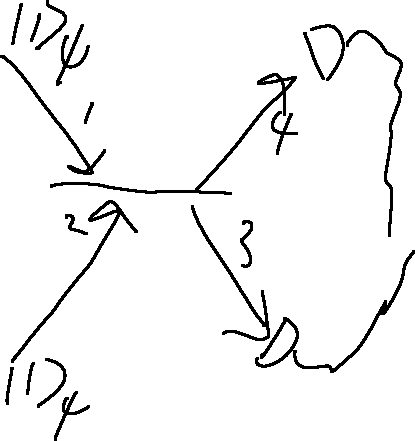
\includegraphics[width=6cm]{2-12-1.png}
	\caption*{Hong-Oh-Mandel}
\end{figure*}
We can see that probability of getting a  coincidence here is:
\begin{align*}
	P &\propto \expval{\hat{a}^\dagger_3\hat{a}_3\hat{a}^\dagger_4\hat{a}_4}
\end{align*}
We can look at this probability by propogating our states, starting with:
\begin{align*}
	\ket{\psi}_\text{in} &= \hat{a}^\dagger_{\psi1}\hat{a}^\dagger_{\psi2}\vac
\end{align*}
And we find that the output is then:
\begin{align*}
	\ket{\psi}_\text{out} &= \frac{1}{2} \left(\hat{a}_{\psi3}^\dagger + \hat{a}_{\psi4}^\dagger\right)\left(\hat{a}_{\psi3}^\dagger - \hat{a}_{\psi4}^\dagger\right)\vac \\
	\ket{\psi}_\text{out} &= \frac{\sqrt{2}}{2} \left(\ket{2}_{\psi3} + \ket{2}_{\psi4}\right)
\end{align*}
Which shockingly gives us either 2 photons at one detector, or two photons at the other, and never a coincidence!
In hindsight this is what we should expect, as bosons tend to clump together. In contrast if we fired two fermions into a beamsplitter like this we would expect to find the electrons never arriving at the same port.

\begin{figure*}[h]
	\centering
	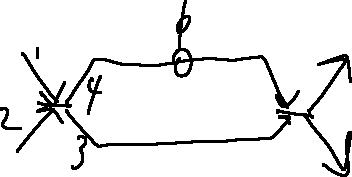
\includegraphics[width=6cm]{2-12-2.png}
	\caption*{NOON interferemoter}
\end{figure*}
Repeating this experement with an additional interference, and a phase we find our coincidence count is:
\begin{align*}
	P &\propto \frac{1-\cos2\phi}{2}
\end{align*}
Which gives us a more sensative measurement of our phase! This is because at the first beamsplitter we have prepared a NooN state.
